% ============================================================
% Section: Method
% ============================================================
\section{Method}
\label{sec:method}

This section presents the mathematical formulation of the benchmark problem and the analytical solution procedure used to generate the reference solution for the FaMoU evolutionary framework.

% ----------------------------------------------------------
\subsection{Two-Group Neutron Diffusion Equations}
\label{sec:two-group}

We consider the steady-state two-group neutron diffusion model on the square domain $\Omega = [-0.5,\, 0.5]^2$:
\begin{align}
  -D_1 \nabla^2 \varphi_1 + \Sigma_r \varphi_1
    &= \nu\Sigma_{f1}\,\varphi_1 + \nu\Sigma_{f2}\,\varphi_2,
    \label{eq:fast-group} \\[4pt]
  -D_2 \nabla^2 \varphi_2 + \Sigma_{a2}\,\varphi_2
    &= \Sigma_{1\to 2}\,\varphi_1,
    \label{eq:thermal-group}
\end{align}
where $\varphi_1(x,y)$ and $\varphi_2(x,y)$ denote the fast and thermal neutron fluxes, respectively, with physical parameters as specified in Table~\ref{tab:params}.

The boundary conditions impose an inhomogeneous incoming current on the left face and reflective (zero Neumann) conditions on the remaining three faces:
\begin{align}
  -D_i\,\frac{\partial\varphi_i}{\partial x}\bigg|_{x=-0.5} &= y,
  \qquad i=1,2,
  \label{eq:bc-left} \\
  \frac{\partial\varphi_i}{\partial x}\bigg|_{x=0.5} &= 0,
  \label{eq:bc-right} \\
  \frac{\partial\varphi_i}{\partial y}\bigg|_{y=\pm 0.5} &= 0.
  \label{eq:bc-topbot}
\end{align}

% ----------------------------------------------------------
\subsection{Fourier Eigenfunction Expansion}
\label{sec:fourier-expansion}

The homogeneous Neumann conditions~\eqref{eq:bc-topbot} in the $y$-direction motivate a Fourier cosine expansion:
\begin{equation}
  \varphi_i(x,y) = \sum_{n=0}^{\infty} \Phi_{i,n}(x)\,
  \cos\!\bigl(n\pi(y+0.5)\bigr),
  \qquad i=1,2.
  \label{eq:fourier-expansion}
\end{equation}
The basis functions $Y_n(y) = \cos\bigl(n\pi(y{+}0.5)\bigr)$ satisfy $Y_n'(-0.5) = Y_n'(0.5) = 0$, thereby enforcing the top and bottom boundary conditions exactly for every truncation order.

Rearranging~\eqref{eq:fast-group}--\eqref{eq:thermal-group} with the coupling coefficients
\begin{equation}
  A_{11} = \Sigma_r - \nu\Sigma_{f1} = 0.0075,\quad
  A_{12} = -\nu\Sigma_{f2} = -0.25,\quad
  A_{21} = -\Sigma_{1\to 2} = -0.015,\quad
  A_{22} = \Sigma_{a2} = 0.1,
  \label{eq:coupling-coeffs}
\end{equation}
and substituting~\eqref{eq:fourier-expansion} into the PDEs yields, for each mode~$n$, a coupled ODE system in $x$.

% ----------------------------------------------------------
\subsection{Coupled ODE System per Mode}
\label{sec:coupled-ode}

Defining $\kappa_n = n\pi$ and the mode-dependent diagonal terms
\begin{equation}
  B_{11}^{(n)} = D_1\kappa_n^2 + A_{11},\qquad
  B_{22}^{(n)} = D_2\kappa_n^2 + A_{22},
  \label{eq:B-coeffs}
\end{equation}
the Fourier-projected system reads
\begin{align}
  -D_1\,\Phi_{1,n}''(x) + B_{11}^{(n)}\,\Phi_{1,n}(x) + A_{12}\,\Phi_{2,n}(x) &= 0,
  \label{eq:ode-fast} \\
  A_{21}\,\Phi_{1,n}(x) - D_2\,\Phi_{2,n}''(x) + B_{22}^{(n)}\,\Phi_{2,n}(x) &= 0.
  \label{eq:ode-thermal}
\end{align}

Seeking solutions of the form $\Phi_{i,n}(x) = a_i\,e^{\alpha x}$ leads to the eigenvalue problem
\begin{equation}
  \begin{pmatrix}
    -D_1\alpha^2 + B_{11}^{(n)} & A_{12} \\[2pt]
    A_{21} & -D_2\alpha^2 + B_{22}^{(n)}
  \end{pmatrix}
  \begin{pmatrix} a_1 \\ a_2 \end{pmatrix} = \mathbf{0}.
  \label{eq:eigenvalue-system}
\end{equation}
Setting the determinant to zero and substituting $\beta = \alpha^2$ yields a quadratic in~$\beta$:
\begin{equation}
  D_1 D_2\,\beta^2
  - \bigl(D_1 B_{22}^{(n)} + D_2 B_{11}^{(n)}\bigr)\,\beta
  + \bigl(B_{11}^{(n)} B_{22}^{(n)} - A_{12}\,A_{21}\bigr)
  = 0.
  \label{eq:characteristic}
\end{equation}
The two roots $\beta_1^{(n)}, \beta_2^{(n)}$ determine the functional form of the $x$-dependent solutions:
\begin{equation}
  f_j(x) =
  \begin{cases}
    \cosh\!\bigl(\!\sqrt{\beta_j}\,(x - 0.5)\bigr)
      & \text{if } \beta_j \geq 0, \\[4pt]
    \cos\!\bigl(\!\sqrt{-\beta_j}\,(x - 0.5)\bigr)
      & \text{if } \beta_j < 0,
  \end{cases}
  \label{eq:basis-functions}
\end{equation}
where the shift by $x_0 = 0.5$ ensures that $f_j'(0.5) = 0$, satisfying the right boundary condition~\eqref{eq:bc-right} by construction.

The eigenvector ratio for each root is
\begin{equation}
  r_j^{(n)} = \frac{a_2}{a_1}\bigg|_{\beta_j}
  = \frac{D_1\beta_j^{(n)} - B_{11}^{(n)}}{A_{12}}.
  \label{eq:eigenvector-ratio}
\end{equation}

The general solution for mode $n$ is therefore
\begin{align}
  \Phi_{1,n}(x) &= C_A^{(n)}\,f_1^{(n)}(x) + C_B^{(n)}\,f_2^{(n)}(x),
  \label{eq:phi1n} \\
  \Phi_{2,n}(x) &= C_A^{(n)}\,r_1^{(n)}\,f_1^{(n)}(x)
                  + C_B^{(n)}\,r_2^{(n)}\,f_2^{(n)}(x).
  \label{eq:phi2n}
\end{align}

% ----------------------------------------------------------
\subsection{Coefficient Determination}
\label{sec:coefficient-determination}

The remaining unknowns $C_A^{(n)}, C_B^{(n)}$ are fixed by the left boundary condition~\eqref{eq:bc-left}. Expanding the forcing term $y$ in the same cosine basis:
\begin{equation}
  y = \sum_{n=1,3,5,\ldots}^{\infty}
  c_n\,\cos\!\bigl(n\pi(y+0.5)\bigr),
  \qquad
  c_n = -\frac{4}{(n\pi)^2} \;\;\text{for odd } n,
  \label{eq:fourier-coeff}
\end{equation}
with $c_n = 0$ for even $n$ and $c_0 = 0$. Only the odd Fourier modes contribute, reflecting the anti-symmetry of the linear source $y$ about the midpoint of the domain.

For each odd mode $n$, equating the Fourier coefficients of the left boundary condition gives the $2\times 2$ linear system:
\begin{equation}
  \underbrace{
  \begin{pmatrix}
    -D_1\,f_1'^{(n)}(-\tfrac12) & -D_1\,f_2'^{(n)}(-\tfrac12) \\[4pt]
    -D_2\,r_1^{(n)}\,f_1'^{(n)}(-\tfrac12)
      & -D_2\,r_2^{(n)}\,f_2'^{(n)}(-\tfrac12)
  \end{pmatrix}
  }_{\mathbf{M}^{(n)}}
  \begin{pmatrix} C_A^{(n)} \\ C_B^{(n)} \end{pmatrix}
  =
  \begin{pmatrix} c_n \\ c_n \end{pmatrix},
  \label{eq:coefficient-system}
\end{equation}
which is solved independently for each retained mode.

% ----------------------------------------------------------
\subsection{Convergence Properties}
\label{sec:convergence}

The Fourier coefficients decay as $c_n = O(n^{-2})$, guaranteeing algebraic convergence of the series~\eqref{eq:fourier-expansion}. In practice, truncating to $N$ odd modes suffices for high-precision reference solutions. Figure~\ref{fig:convergence} shows the RMS PDE and BC residuals versus $N$ under the unified evaluator: the PDE residual remains near $3 \times 10^{-5}$ from the first few modes onward (bounded by the $h = 10^{-6}$ finite-difference precision floor) while the BC residual decreases monotonically to $O(10^{-3})$. At $N{=}30$, the combined score is 0.9989, providing an accurate seed program for FaMoU evolution.

\begin{figure}[t]
  \centering
  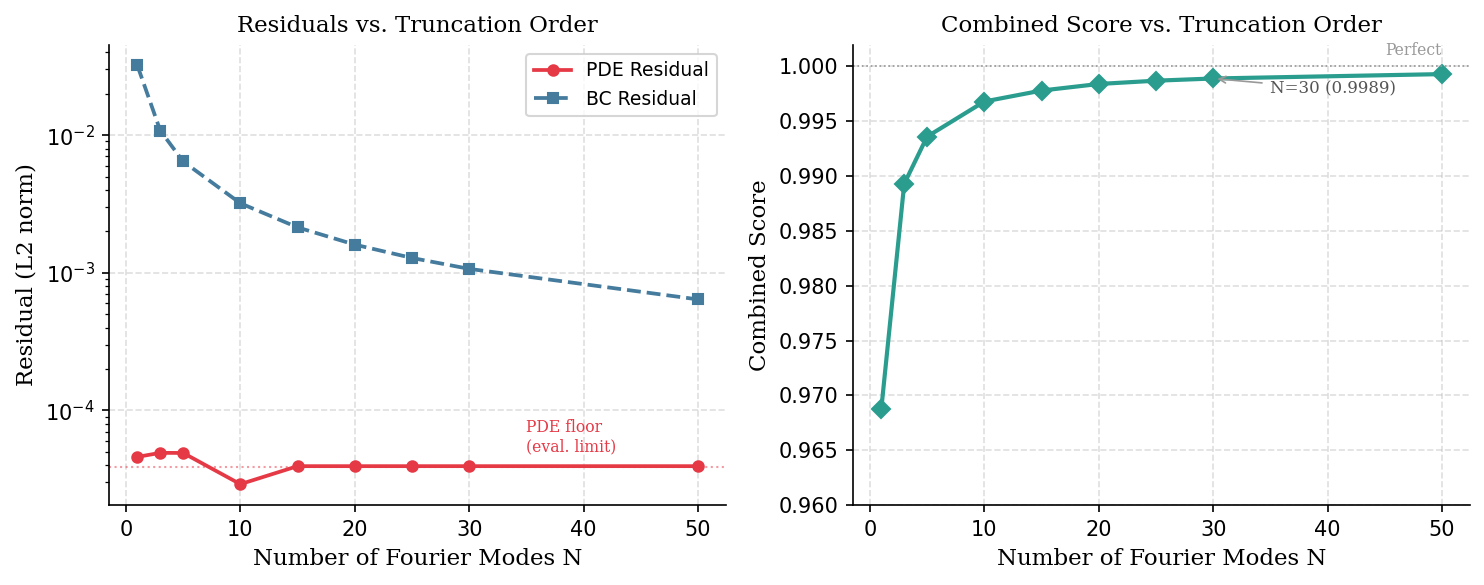
\includegraphics[width=0.65\textwidth]{figs/fig_convergence.png}
  \caption{Convergence of the Fourier expansion. The BC residual (RMS over 40 scalar values) decreases monotonically with the number of retained odd modes~$N$; the PDE residual fluctuates near the $h = 10^{-6}$ finite-difference precision floor ($\sim 3 \times 10^{-5}$) from the first few modes onward.}
  \label{fig:convergence}
\end{figure}

% ----------------------------------------------------------
\subsection{FaMoU: LLM-Driven Program Evolution}
\label{sec:famou}

While the Fourier analytical solution achieves high accuracy (score $= 0.9989$ with $N{=}30$ modes), \textbf{FaMoU} (\underline{Fa}st \underline{Mo}de m\underline{U}tation) further optimizes the numerical implementation through LLM-guided program evolution, exploring solution strategies that may be difficult for human experts to discover manually.

\paragraph{Evolution Loop.}
FaMoU operates as an iterative program synthesis pipeline (Figure~\ref{fig:evolution}):
\begin{enumerate}
  \item \textbf{Initialization.} A seed program (\texttt{init.py}) encodes a baseline analytical solution, e.g., the truncated Fourier expansion with a fixed number of modes.
  \item \textbf{Evaluation.} The evaluator (\texttt{evaluator.py}) computes PDE and boundary-condition residuals at prescribed test points and returns a combined fitness score.
  \item \textbf{LLM Mutation.} A large language model receives the current best program, its fitness score, and a task-specific prompt describing the physics. The LLM proposes modified programs that may adjust the truncation order, refine coefficient computations, or introduce alternative solution representations.
  \item \textbf{Selection.} Candidate programs are ranked by their combined score; the top-performing variant becomes the parent for the next generation.
  \item \textbf{Iteration.} Steps 2--4 repeat for up to $R$ rounds or until the score exceeds a convergence threshold.
\end{enumerate}

\paragraph{Search Space.}
The search space encompasses the full Python program implementing the \texttt{solution(x, y)} interface. Viable mutations include adjusting the number of Fourier modes~$N$, modifying numerical precision strategies (e.g., switching from \texttt{float64} to extended-precision arithmetic), restructuring the eigenvalue solver, or introducing hybrid representations that combine analytical and numerical components. The LLM's capacity for semantic code understanding enables it to navigate this combinatorial space more efficiently than random perturbation.

\paragraph{Evaluation Metric.}
Each candidate program is scored using the combined metric:
\begin{equation}
  S = \frac{1}{1 + \bar{R}_{\mathrm{PDE}} + \bar{R}_{\mathrm{BC}}},
  \label{eq:combined-score}
\end{equation}
where $\bar{R}_{\mathrm{PDE}}$ and $\bar{R}_{\mathrm{BC}}$ denote the root-mean-square (RMS) residuals over the interior test points (8 scalars: 2 equations $\times$ 4 test points) and boundary evaluation points (40 scalars: 2 groups $\times$ 4 faces $\times$ 5 points), respectively. A hard constraint requires $S > 0$ (validity); programs that raise exceptions or produce \texttt{NaN} values receive $S = 0$.

\begin{figure}[t]
  \centering
  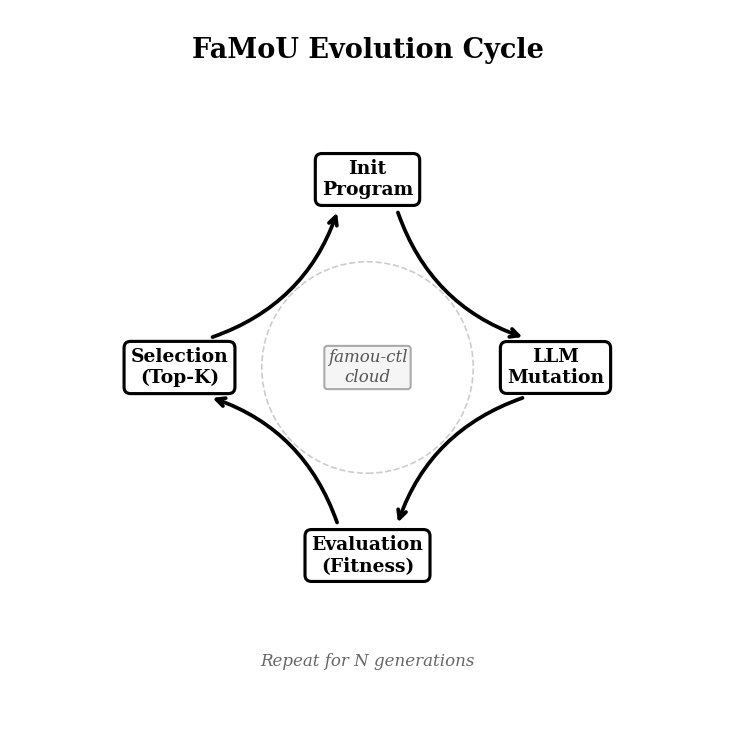
\includegraphics[width=0.85\linewidth]{figs/fig_evolution.png}
  \caption{The FaMoU evolutionary program synthesis loop. Starting from the Fourier analytical seed program, an LLM iteratively mutates solver code guided by automated fitness scores from the physics evaluator.}
  \label{fig:evolution}
\end{figure}
